\documentclass[18pt,compress,ngerman,utf8,t,xcolor=table]{beamer}
\usepackage{etex}
\usepackage[ngerman]{babel}
\usepackage{graphicx}
\usepackage[export]{adjustbox}
\usepackage{multicol}


\usetheme[numbering=fraction, progressbar=frametitle]{metropolis}


\date{\today}
\institute{Student of Rationality}
\graphicspath{ {./template/} {./lesswrong/graphics/} }
% \titlegraphic{\vspace{4cm} \hspace{9cm} \includegraphics[height=2cm]{template/Logo-LessWrong.png}}

\title{How to be less wrong}
\author{Felix Karg}

\newif\ifEnglish
\Englishfalse
% \Englishtrue

\AtBeginSection[]
{
    \Large
    \begin{frame}{Inhalt}
        \tableofcontents[currentsection]
        \clearpage
    \end{frame}
}

\AtBeginSubsection[]
{
    \Large
    \begin{frame}{Inhalt}
        \tableofcontents[currentsection,currentsubsection]
        \clearpage
    \end{frame}
}

% \vspace{0.1cm}



\newcommand{\code}[1]{
    \begin{center}
    \setlength{\fboxrule}{1pt}
    \setlength{\fboxsep}{8pt}
        {\fbox{\parbox{0.81\textwidth}{#1}}}
   \end{center}
}




\begin{document}

\maketitle

% multicols from:
% https://tex.stackexchange.com/questions/24343/splitting-toc-into-two-columns-on-single-frame-in-beamer

%%%%%%%%%%%%%%%%%%%%%%%%%%%%%%%%%%%%%%%%%%%%%%%%%%%%%%%%%%%%%%%%%%%%%%%%%%%%%%%%%%%%%%%%%%%%%%%%%%%%%%%%%%%%%%%%%%%

\begin{frame}{Inhalt}
    \Large
    \tableofcontents[]
\end{frame}




%%%%%%%%%%%%%%%%%%%%%%%%%%%%%%%%%%%%%%%%%%%%%%%%%%BEGINNING
% % \section{Examples}

\begin{frame}[c]
     Here a citation: \cite{benchcpp}
\end{frame}

\begin{frame}[c]{Example slide}
    \Large
    \begin{itemize}[<+->]
        \item First Element
        \item Second Element
        \item Third Element
    \end{itemize}
\end{frame}

\begin{frame}[c]{Other example slide}
    \Large
    \begin{itemize}[<+(1)->]
        \item First Element
        \item Second Element
        \item Third Element
    \end{itemize}
\end{frame}

\begin{frame}[c]{Yet another example slide}
    \Large
    \begin{itemize}
        \item First Element
            \pause
        \item Second Element
            \pause
        \item Third Element
    \end{itemize}
\end{frame}









%
% Wenn die Leute aus dem Vortrag herausgehen, sollen sie mitgenommen haben:
% - bewusstsein schaffen für eigene betroffenheit
% - interesse schaffen sich daran sich damit auseinanderzusetzen -> 
% - 
% Auf jeder Folie etwas vermitteln das nicht auf der Folie steht


\ifEnglish


\begin{frame}[c]{What is Rationality about?}
    Testframe
\end{frame}

% \begin{frame}[standout]
%     Rationality is {\emph about} winning.
% \end{frame}


\else

\section{Was ist Rationalität?}

\begin{frame}[c]{Was ist Rationalität?}
    \Large
    Grob:
    \newline
    \begin{itemize}
    \pause
    \item Die Welt verstehen    \only<3->{(Epistemic Rationality)}
    \newline
    \pause
    \pause
    \item Ziele erreichen       \only<5->{(Instrumental Rationality)}
    \newline
    \end{itemize}
    \pause
    \pause
    Kurz: Rationalität entwickelt unsere Entscheidungen bezüglich Denken und Handeln weiter.
\end{frame}


\begin{frame}[c]{Was ist Rationalität?}
    \Large
    Nutzen von hilfreichen Erkenntnissen aus anderen Bereichen, z.B.:
    \begin{itemize}
    \pause
    \item Bayes' Theorem        \only<3->{(Statistik)}
    \pause
    \pause
    \item Modelle               \only<5->{(Philosophie)}
    \pause
    \pause
    \item Occams Rasiermesser   \only<7->{(Entscheidungstheorie)}
    \pause
    \pause
    \item System I/II           \only<9->{(Kognitionswissenschaften)}
    \pause
    \pause
    \item Rätselhafte Antworten \only<11->{(...)}
    \end{itemize}
\end{frame}

% Wertetheorie, Erkenntnistheorie, Metaphysik

\begin{frame}[c]{Was tun mit den Erkenntnissen?}
    \Large
    \pause
    Optimieren von ...
    \begin{itemize}
    \pause
    \item Strukturen
    \pause
    \item Denkprozessen
    \pause
    \item Verfahrensprozessen
    \pause
    \item ...
    \end{itemize}
\end{frame}





\fi
 % actual introduction, ~85%
\section{Entscheidungsprozesse}

\begin{frame}[c]{Fehlerquellen in Entscheidungsprozessen}
    \centering
    % Folie langsam aufbauen, ist sonst zu viel information auf einmal
    % Konkretes Beispiel!!
    % ideen: Kaufen eines Produktes im Supermarkt
    % idee: Terminoptimierung - Freizeitoption A oder B, fokus auf Gruppendynamik
    \only<1>{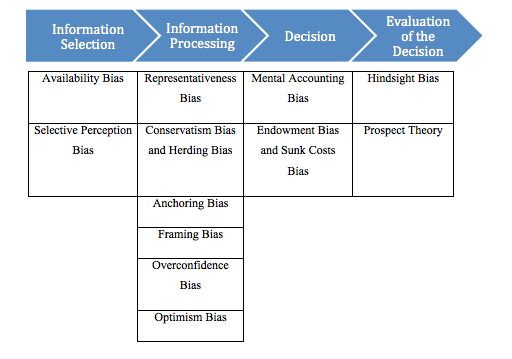
\includegraphics[width=\textwidth, clip=true, trim= 0mm 102mm 0mm 0mm]{DecisionMakingProcedure}}
    \only<2>{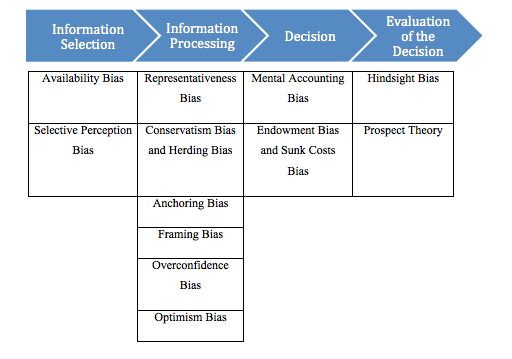
\includegraphics[width=\textwidth]{DecisionMakingProcedure}}
\end{frame}


\begin{frame}[standout]
    ... und das ist nur ein kleiner Auszug.
\end{frame}

\begin{frame}[c]{List of cognitive Biases}
    \centering
    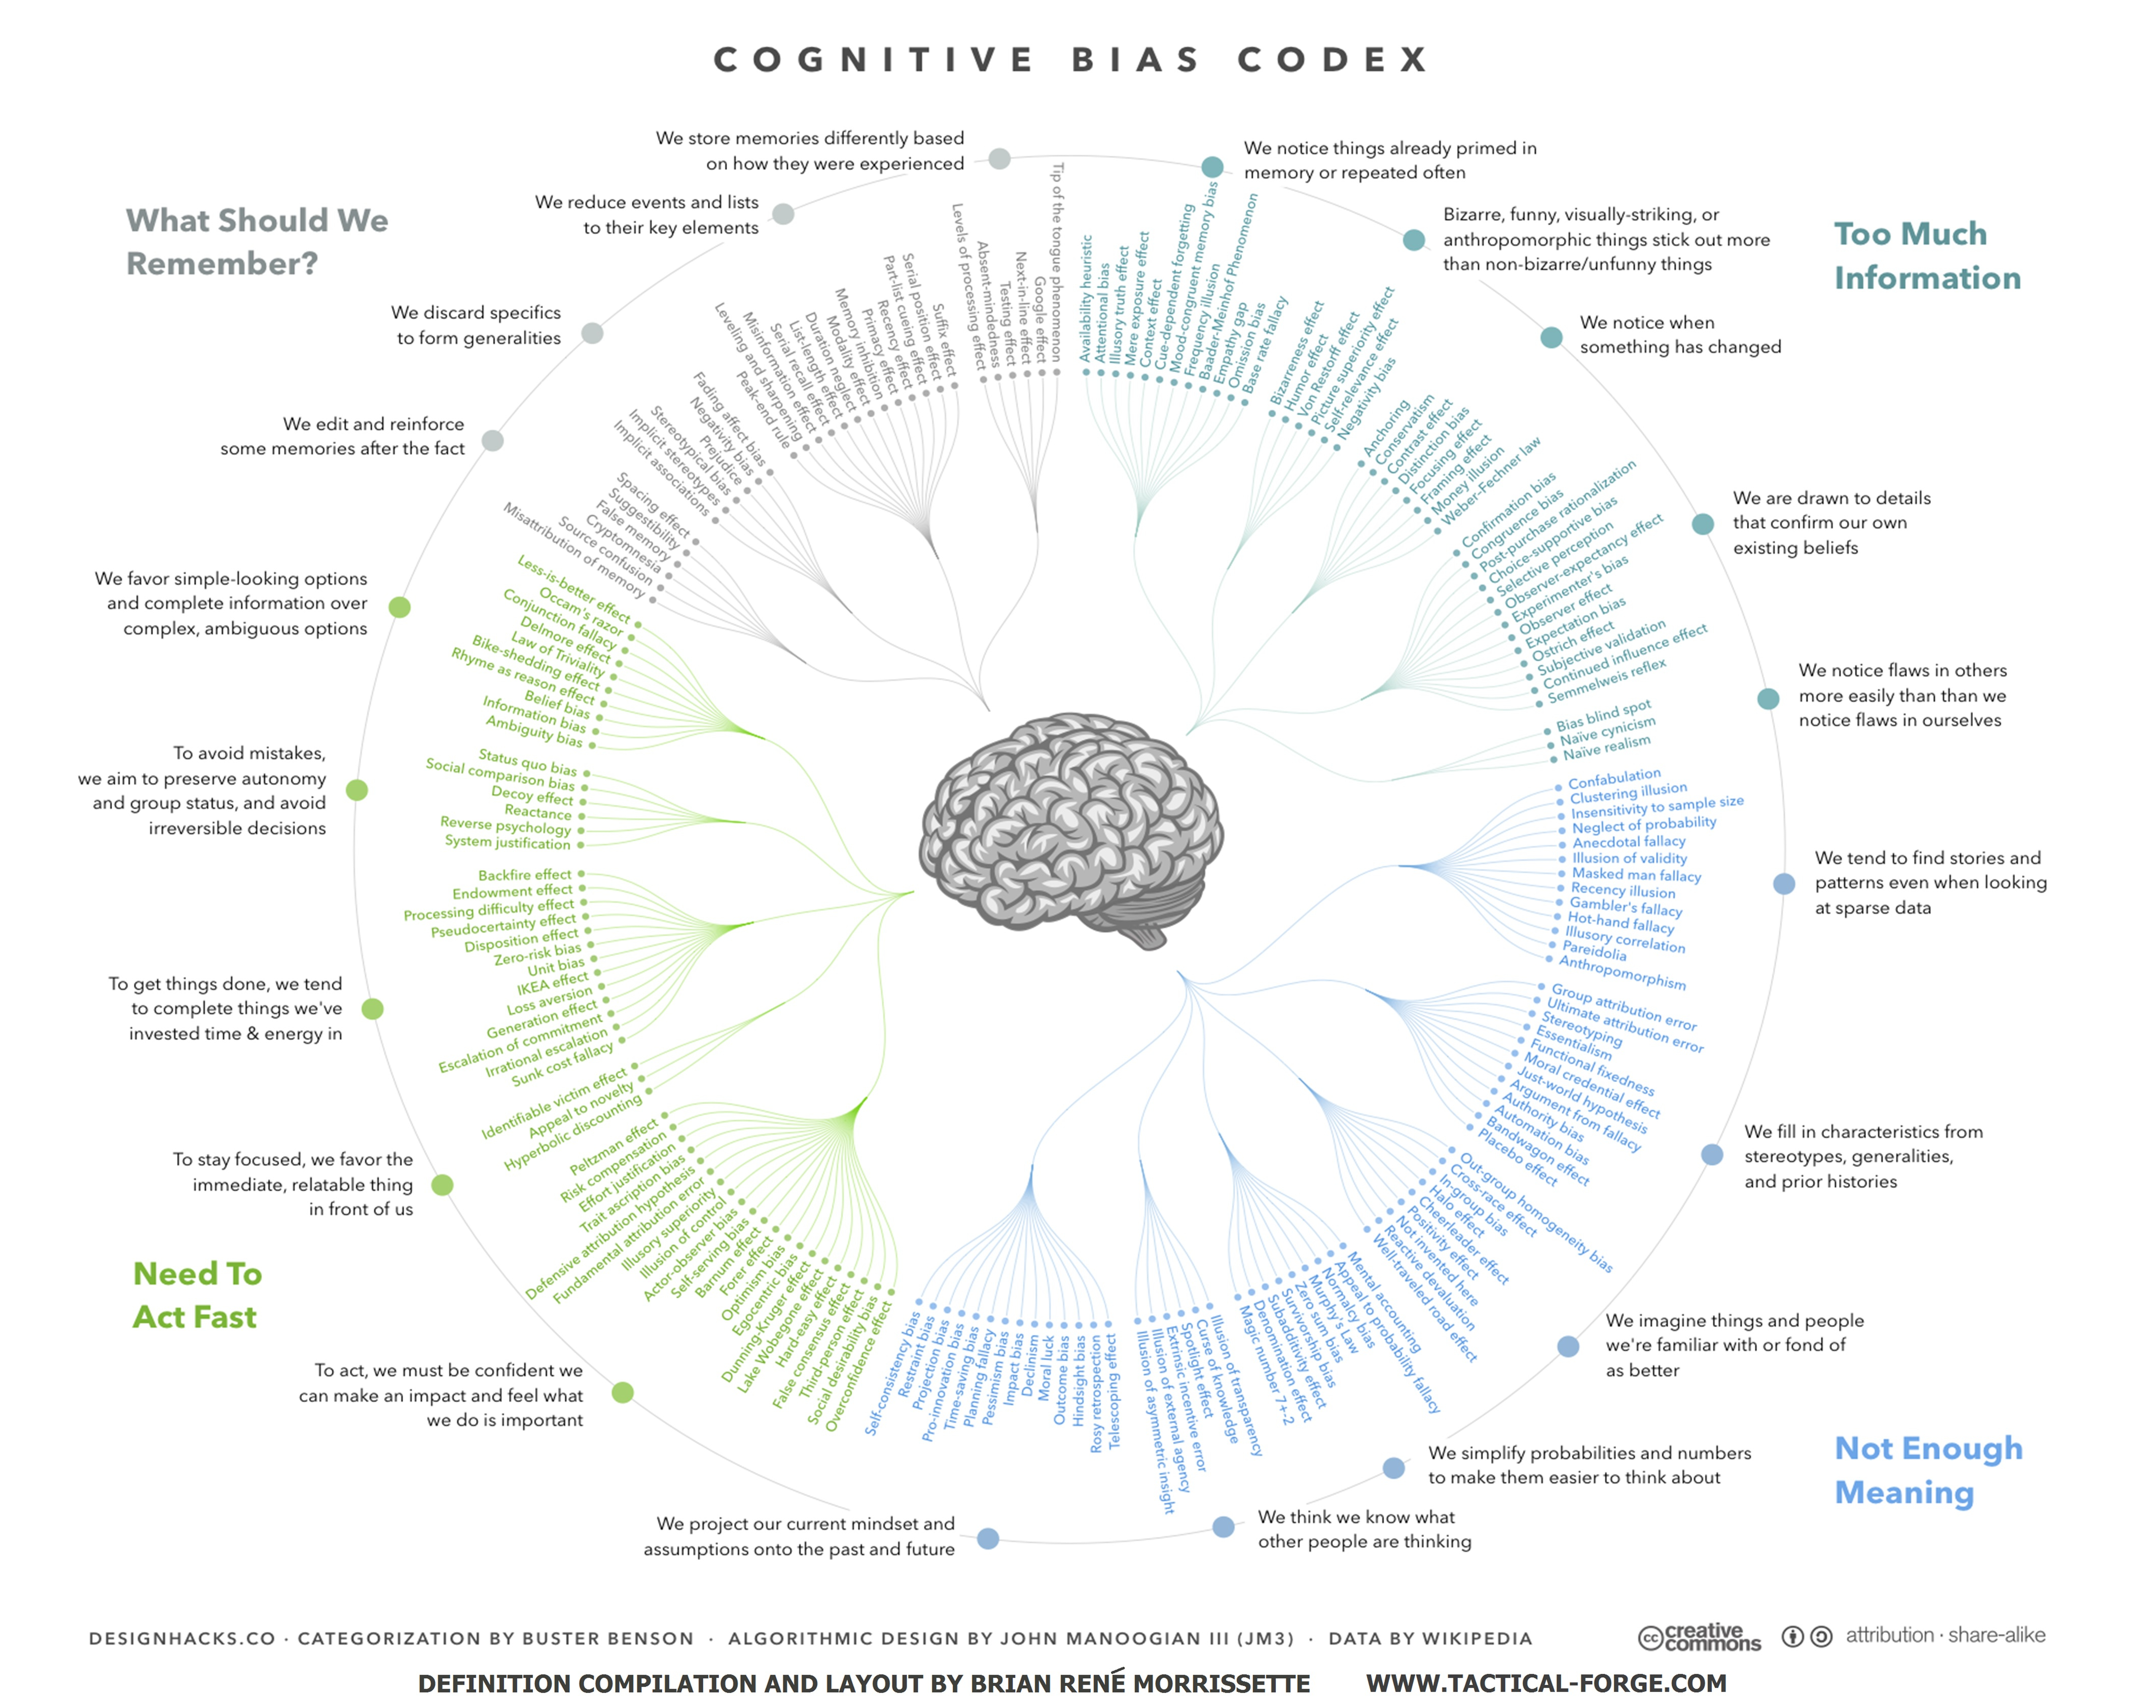
\includegraphics[width=\textwidth]{cogbias_0}
\end{frame}


\begin{frame}[c]{Denken, schnell und langsam}
    \Large
    \pause
    % Das Gehirn arbeitet üblicherweise mit zwei verschiedenen Systemen
    \begin{itemize}
    \item System I - schnelles Denken
    \newline
    \pause
    \item System II - langsames Denken
    \end{itemize}
\end{frame}

     % few slides with a lot of information to talk about
\section{Karte und Gelände}


\begin{frame}[c]{Karte und Gelände}
    \Large
    \pause
    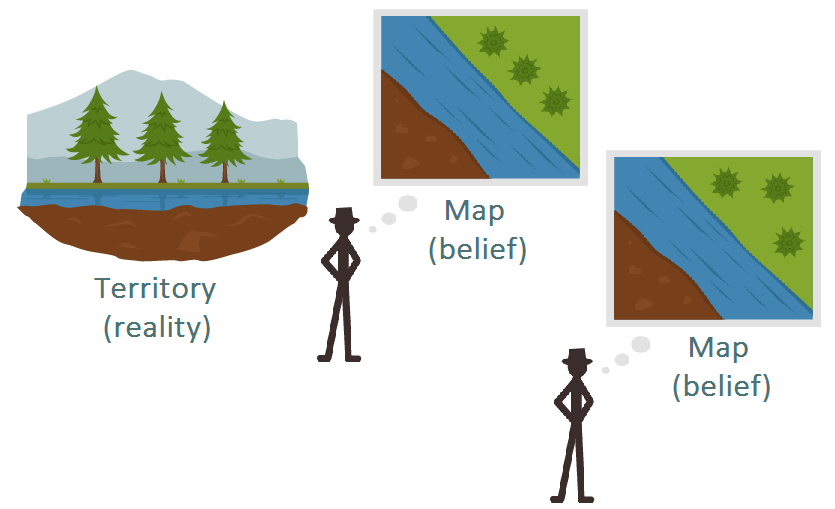
\includegraphics[height=0.85\textheight]{map_territory}
\end{frame}


\begin{frame}[c]{Falsche Erklärungen}
    \only<1>{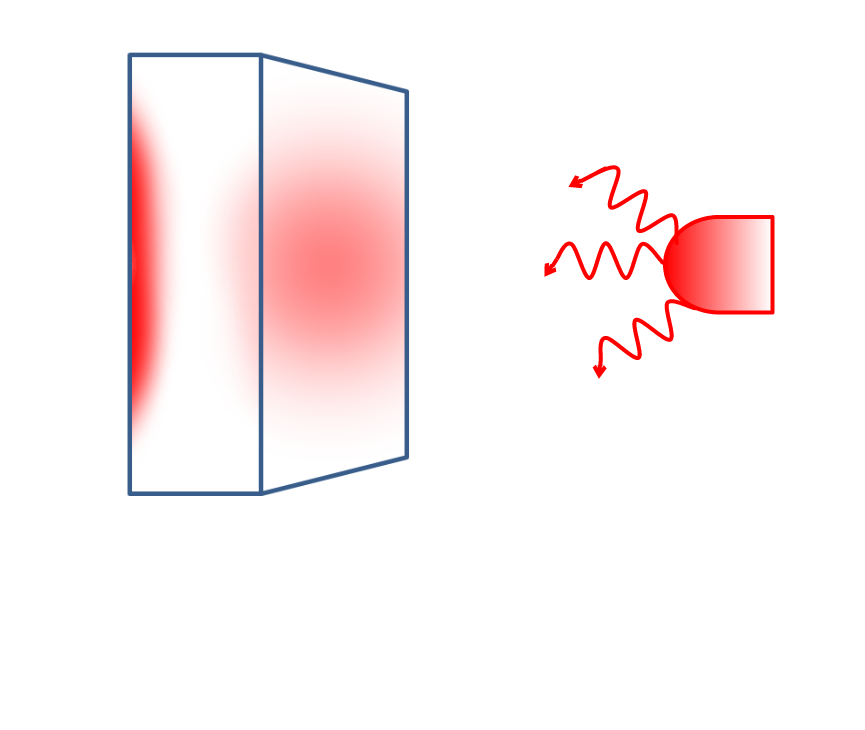
\includegraphics[height=0.95\textheight]{fake_expl_0}}
    \only<2>{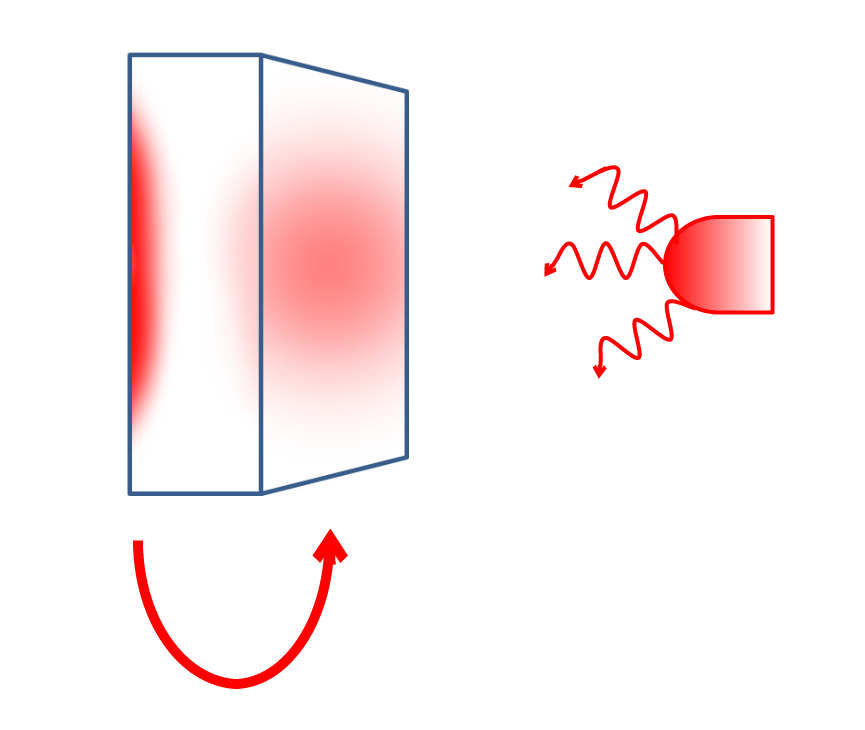
\includegraphics[height=0.95\textheight]{fake_expl_1}}
\end{frame}


\begin{frame}[c]{Eigenschaften eines Rationalisten}
    \Large
    \pause
    Von Fiktion verwirrter zu sein als von der Realität.
    \newline
    \newline
    \pause
    Wenn man jedes Ergebnis gleich gut erklären kann, hat man es nicht verstanden.
\end{frame}





% % % \ifEnglish
%%%%%%%%%%%%%%%%%%%%%%%%%%%%%%%%%%%%%%%%%%%%%%%%%%%%%%%%%%%%

\section{Predictably Wrong}





%%%%%%%%%%%%%%%%%%%%%%%%%%%%%%%%%%%%%%%%%%%%%%%%%%%%%%%%%%%%
\else
%%%%%%%%%%%%%%%%%%%%%%%%%%%%%%%%%%%%%%%%%%%%%%%%%%%%%%%%%%%%

\section{Vorhersagbar Falsch}

\begin{frame}[c]{Unwahrscheinliche Details}
    
\end{frame}





%%%%%%%%%%%%%%%%%%%%%%%%%%%%%%%%%%%%%%%%%%%%%%%%%%%%%%%%%%%%
\fi
     % still exists, won't be used.

\section{Bayes' Theorem}


\begin{frame}[c]{Bayes'sche Theorem: xkcd}
    \begin{multicols}{2}
    \begin{itemize}
        \item[]<1> 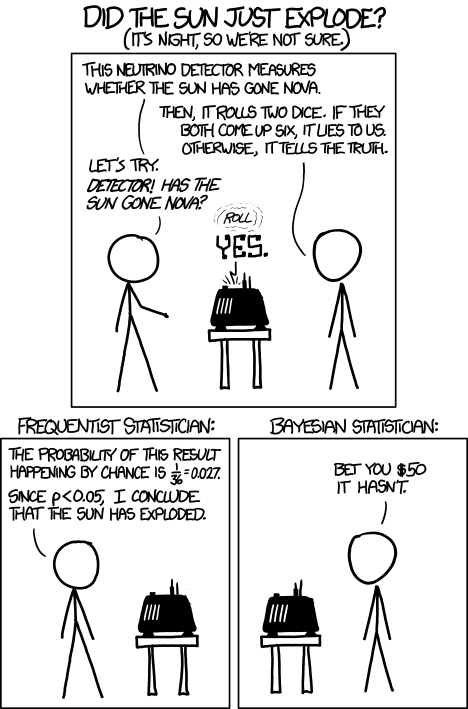
\includegraphics[height=7cm]{strategy/xkcd_frequentists_vs_bayesians.png}
        \item[]<2> 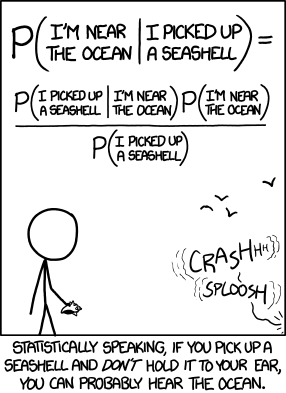
\includegraphics[height=7cm]{strategy/xkcd_seashell.png}
    \end{itemize}
    \end{multicols}
\end{frame}


\begin{frame}[c]{Das Bayes'sche Theorem}
    \Large
    \[
        P(A|X) = \frac{P(X|A) * P(A)}{P(X|A) * P(A) + P(X|\neg A) * P(\neg A)}
    \]
\end{frame}


\begin{frame}[c]{Bayes vs Klassische Stastik}
    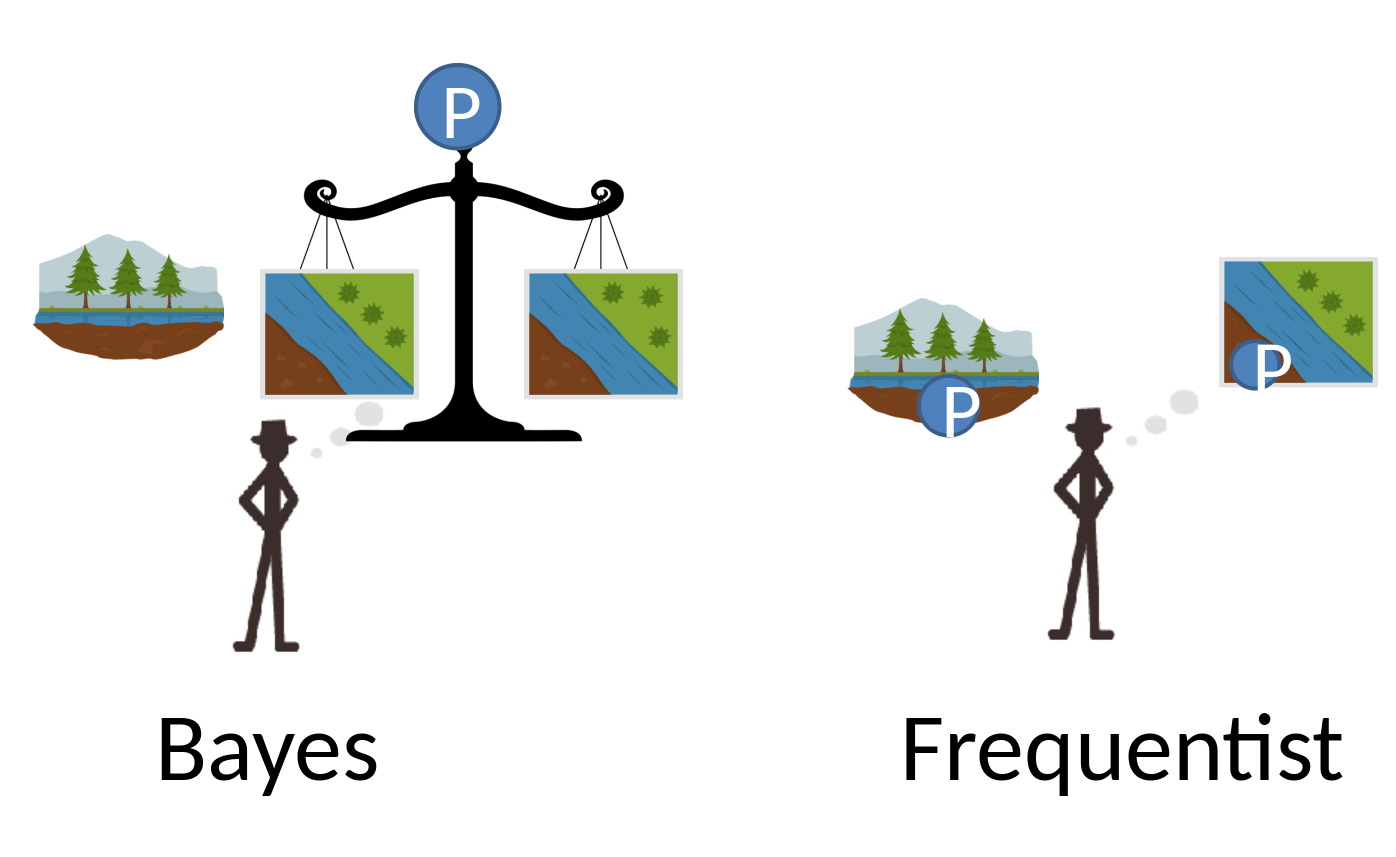
\includegraphics[width=\textwidth]{bayes_vs_freq}
\end{frame}



     % in progress ~20%
\ifEnglish
%%%%%%%%%%%%%%%%%%%%%%%%%%%%%%%%%%%%%%%%%%%%%%%%%%%%%%%%%%%%

\section{Occam's Razor}

\begin{frame}[c]{Occam's Razor - General Description}
    Usually something like this: ...
\end{frame}



%%%%%%%%%%%%%%%%%%%%%%%%%%%%%%%%%%%%%%%%%%%%%%%%%%%%%%%%%%%%
\else
%%%%%%%%%%%%%%%%%%%%%%%%%%%%%%%%%%%%%%%%%%%%%%%%%%%%%%%%%%%%

\section{Occam's Rasiermesser}

\begin{frame}[c]{Occam's Rasiermesser - Allgemeine Beschreibung}
    Üblicherweise sinngemäß so: ...
\end{frame}


%%%%%%%%%%%%%%%%%%%%%%%%%%%%%%%%%%%%%%%%%%%%%%%%%%%%%%%%%%%%
\fi
     % in progress ~85%
\section{Rätselhafte Antworten}

\begin{frame}[c]{Was sind Rätselhafte Antworten?}
    \Large
    \begin{itemize}[<+->]
    \item Liefern gewöhnlicherweise keine Befriedigende Antwort
    \item Aber hindern uns daran weiter nachzufragen (Stoppt Neugier)
    \item vertreter sind üblicherweise stolz auf ihre Ansichten
    \item Hinterher ist man nicht schlauer
    \end{itemize}

\end{frame}




\begin{frame}[c]{Rätselhafte Antworten - Beispiele}
    \Large
    \begin{itemize}[<+->]
    \item Elan vital
    \newline
    \item Phlogiston
    \newline
    \item Wissenschaft
    \newline
    \item ...
    \end{itemize}
\end{frame}


\begin{frame}[c]{Rätselhafte Antworten - Kontern}
    \Large
    \begin{itemize}[<+->]
    \item Wie sehr wäre ich verwirrt, wenn es anders gewesen wäre?
    \newline
    \item Kann ich damit etwas vorhersagen?
    \newline
    \item Ist die Erklärung beser als 'Weil Magie'?
    \newline
    \item Kausalitätsdiagramme zeichnen und Lücken finden
    \end{itemize}
\end{frame}


\begin{frame}[c]{Semantische Stoppschilder}
    \Large
    \begin{itemize}[<+->]
    \item Rätselhafte Antworten
    \newline
    \item 'Dieses Phänomen ist ein Komplexer Prozess'
    \newline
    \item Demokratie
    \newline
    \item Medizin
    \newline
    \item Gott
    \newline
    \item ...
    \end{itemize}
\end{frame}




\begin{frame}[standout]
    Fazit
\end{frame}


 % in progress ~25%
% \input{critical.tex}  % not existent yet


%%%%%%%%%% END %%%%%%%%%%
\ifEnglish
%%%%%%%%%%%%%%%%%%%%%%%%%%%%%%%%%%%%%%%%%%%%%%%%%%%%%%%%%%%%

\section{Sources}

\begin{frame}[c]
    
\end{frame}



%%%%%%%%%%%%%%%%%%%%%%%%%%%%%%%%%%%%%%%%%%%%%%%%%%%%%%%%%%%%
\else
%%%%%%%%%%%%%%%%%%%%%%%%%%%%%%%%%%%%%%%%%%%%%%%%%%%%%%%%%%%%


%%%%%%%%%%%%%%%%%%%%%%%%%%CITES%%%%%%%%%%%%%%%%%%%%%%%%%%%%%
\section{Quellen}

%%%%%%%%%%%%%%%%%%%%%%%%%%CITES%%%%%%%%%%%%%%%%%%%%%%%%%%%%%
\begin{frame}[c,fragile,allowframebreaks]{Quellen}
    Die Folien sind zu finden unter: \newline
    \url{https://github.com/fkarg/things-to-talk-about/tree/master/lesswrong}
    \newline
    \newline
    Das Forum, mit diesen und sehr viel mehr Themen: \newline

% 
% 
%     Das Buch, aus dem ich den Vortrag gebastelt hab:
% 
    \beamertemplatearticlebibitems
    \begin{thebibliography}{10}
    \bibitem{Less Wrong}
            {\bf Less Wrong}
            \newblock \url{http://lesswrong.com/}

%     \beamertemplatebookbibitems
%     \bibitem{Richard Rumelt}
%         Richard Rumelt
%         \newblock {\em Good Strategy / Bad Strategy}.
%         \newblock The Difference and Why It Matters \\
%                   ISBN: 978-1-78125-154-6
%     \beamertemplatearticlebibitems
%     \bibitem{Lesswrong}
%         Lesswrong
%             \newblock {\em Expecting short Inferential Distances}
%             \newblock \url{http://lesswrong.com/lw/kg/expecting\_short\_inferential\_distances/}
%     \bibitem{Lesswrong}
%         Lesswrong
%             \newblock {\em Cached Thoughts}
%             \newblock \url{http://lesswrong.com/lw/k5/cached\_thoughts/}
%     \bibitem{Zenhabits}
%         Zenhabits
%             \newblock {\em say No so you can say YES}
%             \newblock \url{https://zenhabits.net/say-yes/}
% 
%     \bibitem{Wikiquote}
%         Fukuzawa Yukichi
%             \newblock {\em Wikiquote}
%             \newblock \url{https://en.wikiquote.org/wiki/Fukuzawa\_Yukichi}
% 
%     \bibitem{SpaceX}
%         SpaceX
%             \newblock {\em SpaceX}
%             \newblock \url{http://www.spacex.com/}
% 
%    \bibitem{Wihipedia}
%        Wikipedia
%            \newblock {\em Proton-M}
%            \newblock \url{https://en.wikipedia.org/wiki/Proton-M}
%    \bibitem{Wikipedia}
%        Wikipedia
%            \newblock {\em Ariane 5}
%            \newblock \url{https://en.wikipedia.org/wiki/Ariane\_5}
%    \bibitem{Wikipedia}
%        Wikipedia
%            \newblock {\em Delta IV Heavy}
%            \newblock \url{https://en.wikipedia.org/wiki/Delta\_IV}
   \end{thebibliography}
    % required the allowframebreaks for longer lists

\end{frame}



%%%%%%%%%%%%%%%%%%%%%%%%%%%%%%%%%%%%%%%%%%%%%%%%%%%%%%%%%%%%
\fi




% Modelle/Modelltheorie
% relativ theoretisch aber nicht abgehoben
% notwendigerweise vereinfachung

% noticing confusion-bsp:
% 




% conter deklarieren funktioniert so:
% \newcounter{official}
% \setcounter{official}{\value{page}}

%%%%%%%%%%%%%%%%%%%%%%%%%%%%%%%%%%%%%%%%%%%%%%%%%%%%%%%%%%%%%%%%%%%%%%%%%%%%%%%%%%%%%%%%%%%%%%%%%%%%%%%%%%%%%%%%%%%


\end{document}
